The first of the two software packages chosen for performance analysis is FastJet \cite{fastjet_site}. It is the most widely used jet reconstruction software, and for good reasons. An extensive range of jet finding tools and a number of jet substructure utilities, considered in chapter \ref{ch:reconstruction}, are implemented. FastJet is written using C++ and consists of around two million lines of code spread in one thousand different files. Its capabilities are vast, and extend way beyond the scope of this project.

\section{Why FastJet}\label{ch:whyfj}
So, what is it that makes FastJet so loved by the physics community? First of all, its simple interface. All the tools and methods incorporated by FastJet are easily accessed and can be used by writing a few lines of code. Proof of that is the  example code provided in section \ref{ch:fjexample}. Secondly, its flexibility and insensibility. The software is written in such a way that different parts of it can fit together like puzzle pieces and be combined however the user wants. Moreover, there is a very active community of FastJet contributors amongst physicists, implementing new jet algorithms. 

%The difficulty that arises, however, is that at hadron colliders, clustering is often performed with several hundreds or even thousands of particles. Given N particles, there are N(N - 1)/2 dij distances to calculate, and since one must identify the smallest of these O(N2) distances at each of O(N) iterations of the algorithm, original implementations of the kt algorithm [11, 12] involved O (N3) operations to perform the clustering. 

%In practice this translates to about 1 s for N = 1000. Given that events with pileup can have multiplicities significantly in excess of 1000 and that it can be necessary to cluster hundreds of millions of events, N3 timing quickly becomes prohibitive, all the more so in time-critical contexts such as online triggers. 

The third reason that makes FastJet so popular, which may also be the most important, is its speed. The truth is, a few of the FastJet algorithms can be naively implemented in just several lines of code. The difference rises, when the clustering has to be performed with several hundreds or even thousands of particles. 

Simple implementations scale as $O(N^3)$, essentially calculating the smallest distance between any two particles for a number of iterations. These implementations, when put against the vast amount of events to be processed, struggle to keep up. Even more in time sensitive environments, like the ATLAS online trigger system. 

The algorithms included in FastJet, on the other hand, make use of symmetries that exist when calculating the distance between two particles, and use optimised versions of the numerical equations so that some parts of them are constant and do not have to be recalculated on each step. Moreover, many constrains implied by the geometry of the problems are taken into account to make the computations less expensive. Finally, where possible, FastJet utilises external libraries, for example Computational Geometry Algorithms Library (CGAL). Taking into account everything mentioned in this paragraph, FastJet manages to achieve an $O(N^{2}* ln(N))$ scaling \cite{cacciari2012fastjet}.

In order to understand the magnitude of the improvement FastJet provides, for 1000 particles, a naively implemented $O(N^3)$ scaling algorithm would take around $1s$ to calculate the result. On the other hand, FastJet's $O(N^{2}* ln(N))$ scaling can compute that in milliseconds, making it almost 1000 times faster.


\subsection{Choice of algorithmic strategy}\label{ch:fjstrategy}
FastJet contains different ways of implementing each algorithm. Depending on the number of particles and the radius parameter R (how big the final jet should be), FastJet has the freedom to choose which implementation of the algorithm is the most appropriate to use. The user can pass an extra algorithmic \textit{strategy} argument to the clustering function, requesting a specific strategy, but this just acts as a guideline and FastJet is free to ignore it.

Figure \ref{fig:fjstrategy} shows for two clustering algorithms, the anti-kt and Cambridge, the implementation strategy that will most probably be selected depending on the number of particles and the radius (R). The choice of strategy is done for performance reasons. The optimal strategy may vary depending on the system FastJet is being ran on. That is not taken into account of by FastJet though.

\begin{figure}[H]
    \centering
    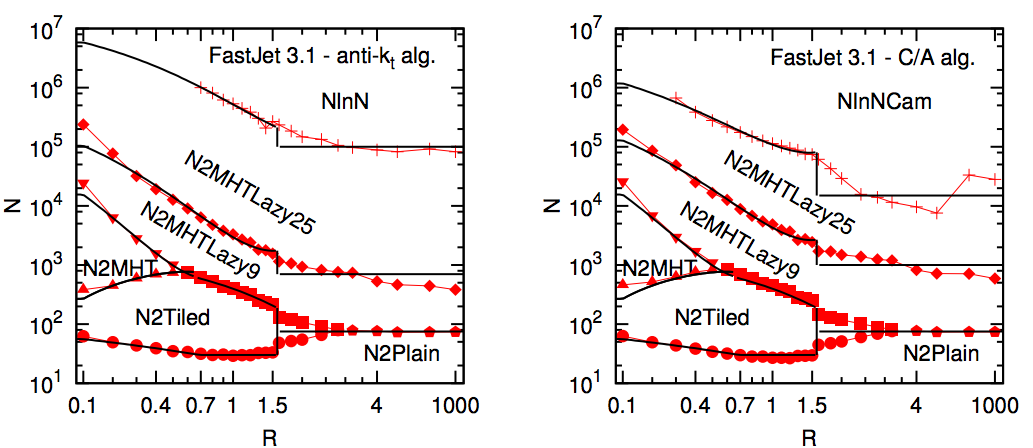
\includegraphics[width=\linewidth]{images/fjstrategy.png}
    \caption{Transitions between chosen strategies in the plane of particle multiplicity N and radius R. The red lines with symbols indicate the measured transitions, while the black solid lines are the
approximate transitions used for the chosen strategy. The left plot is for anti-kt and the right for Cambridge. Taken from \cite{cacciari2012fastjet}.}
    \label{fig:fjstrategy}
\end{figure}


\subsection{Tiled strategy}\label{ch:tiled}
Of the FastJet strategies mentioned, one will directly concern the performance analysis of chapter \ref{ch:workfastjet}, and is thus explained here. When a sequential clustering algorithm iterates through all the particles of the event to find their nearest neighbour, it is rather inefficient to examine the distance to any other particle. For some of them, it is already known that they are far away.

Optimised versions of these algorithms separate the particles in tiles. Depending on the definition of distance for each algorithm, particles that are closer together are put in the same tile. When looking for the nearest neighbour, it is only necessary to examine the particles in the same and neighbouring tiles. Grouping particles in tiles is an extra computational step that has to be taken, but it is done only once at the start of the algorithm and as pairs of particles are merged, it just has to be kept updated.

\section{Installing FastJet}\label{ch:fjtech}
FastJet is available under the GNU public license and can be downloaded from the official FastJet website(\cite{fastjet_site}. In order to be used, FastJet should first be installed on a system. The process includes utilising a configure file, that when run produces a Makefile. In turn, the Makefile can be used to compile the software. The installation process is pretty much straightforward and takes roughly three and a half  minutes on Cirrus\footnote{Cirrus is discussed in section \ref{ch:cirrus}}.  

The default compiler is GNU, the default compiler optimisation flag is -O2, and library linking is dynamic. Those can be changed through arguments on the configure phase of the installation. For example, in order to use the Intel compilers and the -O3 flag, the user can add to the first line:

\begin{lstlisting}
     CC=icc CXX=icpc CXXFLAGS=-O3 CFLAGS="-O3"
\end{lstlisting} 

Many of the algorithms that can be implemented by FastJet are not included in the FastJet built-in functions, but in an open source add-on package called FastJet Contributions \cite{fjcontrib}. The procedure to install this add-on is almost identical to the one followed to install the core FastJet software. The sole difference is that an extra argument has to be passed while configuring, pointing the location of the original FastJet configure file.

\section{Using FastJet}
After the installation, in order to use FastJet, the user is able to write their own C++ code, including the appropriate header file. Then the user's code can be linked to the FastJet libraries and compiled. 

FastJet heavily utilises classes and std:vectors. For basic usage of the software there exist three core classes PseudoJet, JetDefinition and ClusterSequence. For more detailed explanation, refer to chapter 3 of the FastJet manual \cite{cacciari2012fastjet}. Following the definitions a simple example of FastJet usage follows, in order to aid the understanding of FastJet usage.

\subsection{FastJet core classes}
\subsubsection{PseudoJet}\label{ch:pseudojet}
All jets, as well as input particles to the clustering, are PseudoJet objects. The PseudoJet class provides a jet object with a four-momentum and some internal indices to situate it in the context of a jet-clustering sequence.

\subsubsection{JetDefinition}
The class JetDefinition contains a specification of how jet clustering is to be performed. Usually, a "jet definition" instance includes the jet algorithm name, the radius R,  possibly the strategy, and the recombination scheme. 

The Recombination scheme is the way the four-momentum of pseudojets will be combined when these are merged. It can vary from simple addition of the individual components to complex functions.


\subsubsection{ClusterSequence}
To run the jet clustering, the user is required to create a ClusterSequence object. The ClusterSequence class carries out jet-clustering and provides access to the final jets.

\subsection{FastJet example Code}\label{ch:fjexample}
From the bellow example code, in lines \ref{line:A} to \ref{line:B} jets are defined, while in lines \ref{line:C} to \ref{line:D} they are passed to the algorithm.


\lstinputlisting[language=C++,escapechar=|]{codes/example_code.cc}

In order for the code to be compiled, the directory of the installed FastJet files should be pointed out by:

\begin{lstlisting}
g++ example.cc -o example \
     `fastjet-install/bin/fastjet-config --cxxflags --libs --plugins`
\end{lstlisting}